% This file creates beamer slides for the paper Balboni et al 2024 FiFirm Adaptation in Production Networks: Evidence from Extreme Weather Events in Pakistan

\documentclass{beamer}

\usepackage[utf8]{inputenc} % Ensure proper encoding
\usepackage{graphicx} % For including images
\usepackage{hyperref} % For hyperlinks
\usepackage{amsmath,amsfonts,amssymb} % For mathematical symbols and equations

\setbeamertemplate{footline}[frame number] % Add page numbers to each slide

\begin{document}

\title{No margin, no mission? A field experiment on incentives for public
service delivery}
\author{Nava Ashraf, Oriana Bandiera, B. Kelsey Jack}

\institute{Muhammad Bashir}
\date{\today}

\frame{\titlepage}

\begin{frame}{Introduction}
\begin{itemize}
    \item What does motivate people to work and importantly work hard?
    \item Crucial for designing mechanisms to align organizational objectives with individual incentives
    \item The theoretical literature suggests reasons why the effect of extrinsic
    rewards on performance in private and pro-social tasks might differ.
    \item Mission driven organizations hire specific individuals who are intrinsically motivated to work for the organization’s mission. Hence, extrinsic rewards may create negative response as we saw in Benabou and Tirole (2003).

\end{itemize}

\end{frame}

\begin{frame}{This Paper}
\begin{itemize}
    \item To study this, they conduct an experiment to  evaluate the effect of extrinsic rewards, both financial and non-financial, on the performance of agents recruited by a public health organization to promote HIV prevention and sell condoms
    \item The experiment is designed to measure the interaction
    between extrinsic rewards and the pro-social motivation of the agents, and to test whether this interaction differs between financial and nonfinancial rewards.
    
\end{itemize}

\end{frame}

\begin{frame}[allowframebreaks]{Experiment Design}
    \begin{itemize}
        \item They  collaborate with a public health organization
        based in Lusaka, Zambia, which recruits and trains hairdressers and
        barbers to provide information about HIV prevention and sell condoms
        in their shops.
        \item The experiment randomly assigns 205 distinct geographical clusters
        containing 1222 agents to one of four groups that receive different
        rewards based on condom sales. Agents in the control group receive no
        rewards, while agents in the three treatment groups receive financial
        margins at the bottom and the top of the feasible range, and nonfinancial rewards, respectively. The smaller and larger financial-margin
        treatments pay a 10\% and 90\% margin on each condom sale, respectively,
        whereas the non-financial scheme (“star” treatment) gives agents a
        “thermometer” display, showing condom sales and stamps, with one
        star stamp for each sale.        
    \end{itemize}
  
\begin{figure}
    \centering
    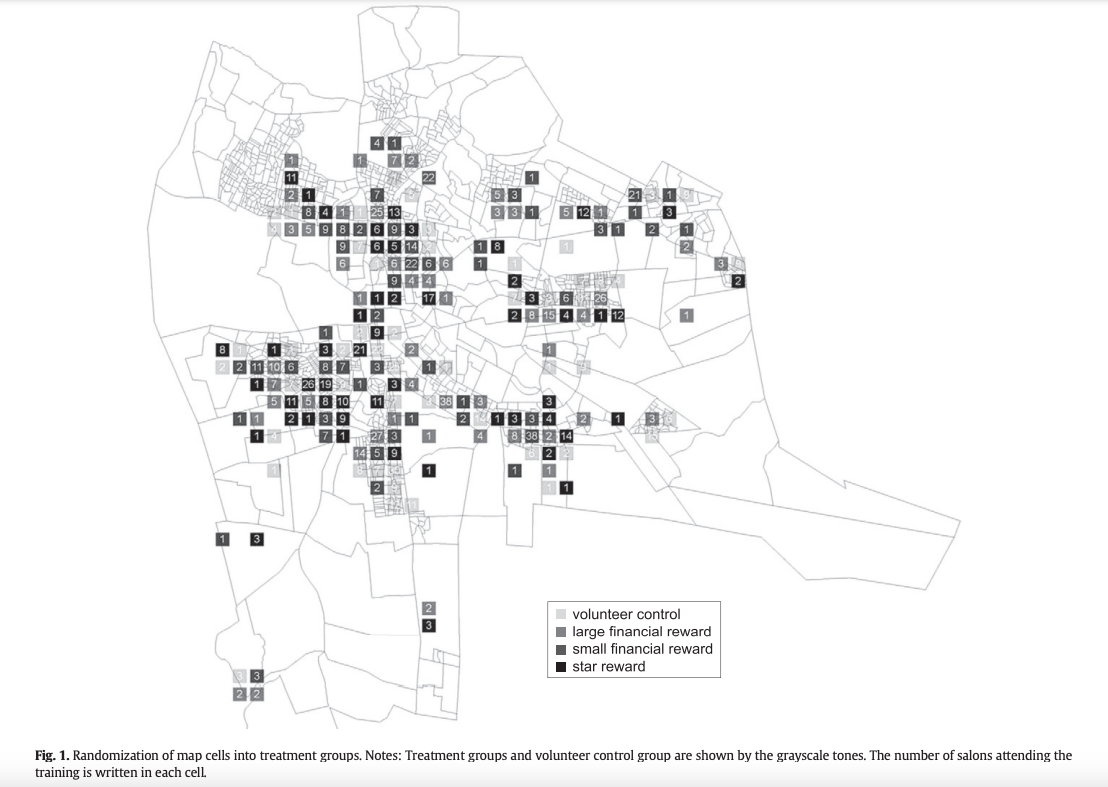
\includegraphics[width=0.8\textwidth]{F1.png}
    \caption{Experiment Design}
    \label{fig:my_label}
\end{figure}
\end{frame}

\begin{frame}{Summary Statistics}
    \begin{figure}
        \centering
        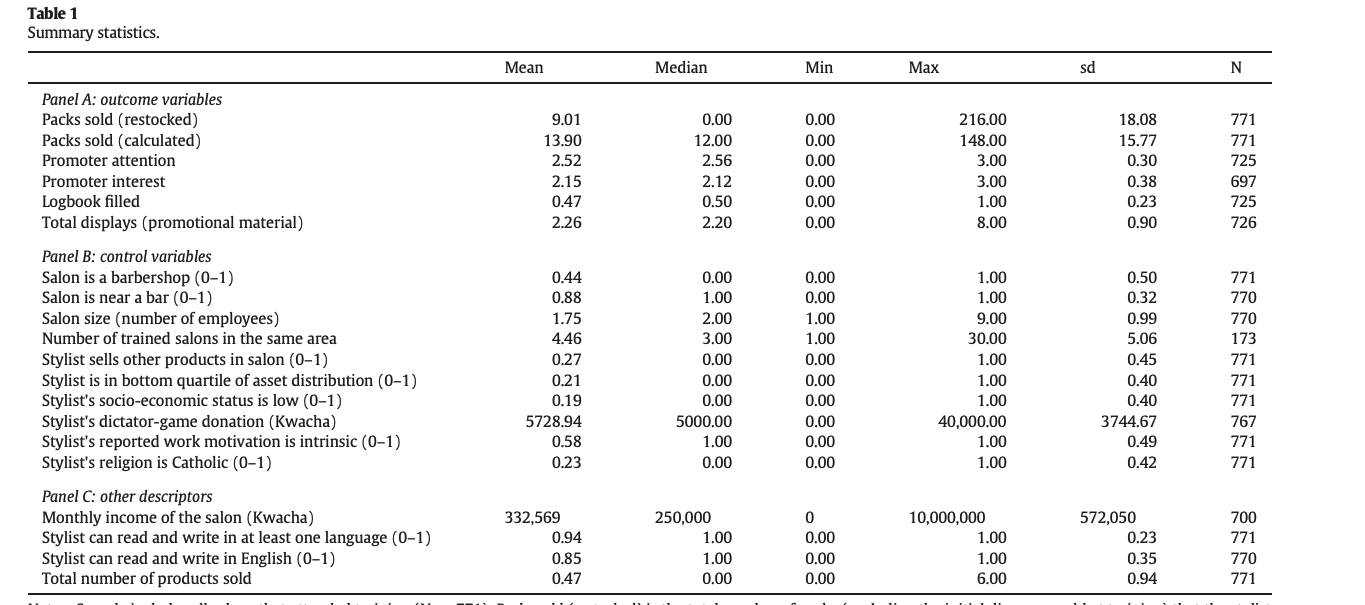
\includegraphics[width=\textwidth]{T1.png}
        \label{fig:my_label}
    \end{figure}




\end{frame}

\begin{frame}{Non-financial Incentives are effective}
    \begin{figure}
        \centering
        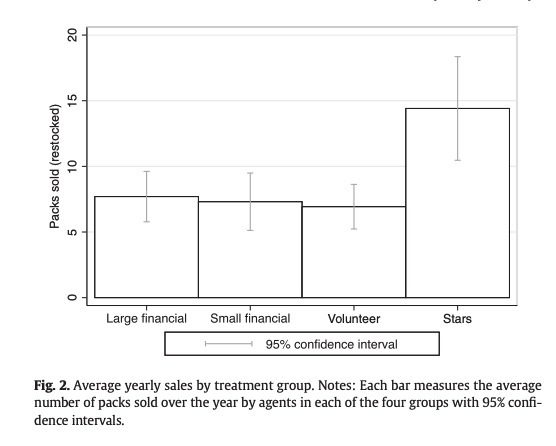
\includegraphics[width=\textwidth]{F2.png}
        \label{fig:my_label}
    \end{figure}
\end{frame}


\begin{frame}{Non-financial Incentives are effective}
    \begin{figure}
        \centering
        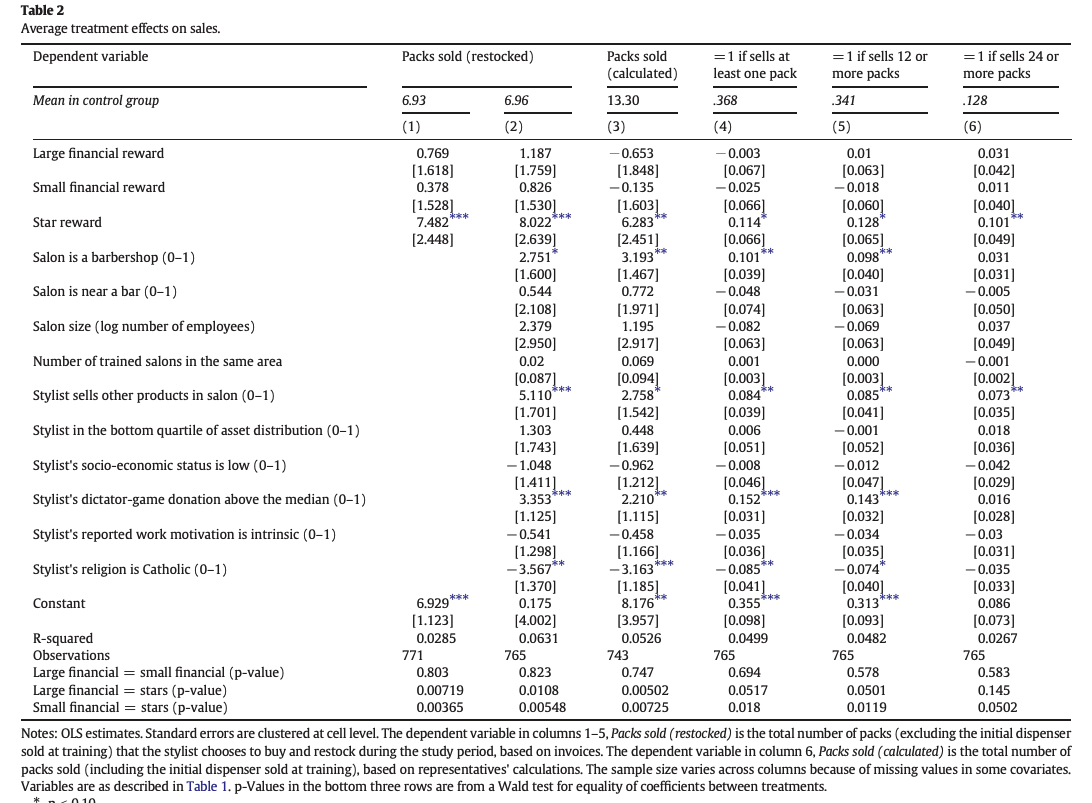
\includegraphics[width=\textwidth]{T2.png}
        \label{fig:my_label}
    \end{figure}
\end{frame}

\begin{frame}{Non-financial Incentives are stable and not driven by novelity}
    \begin{figure}
        \centering
        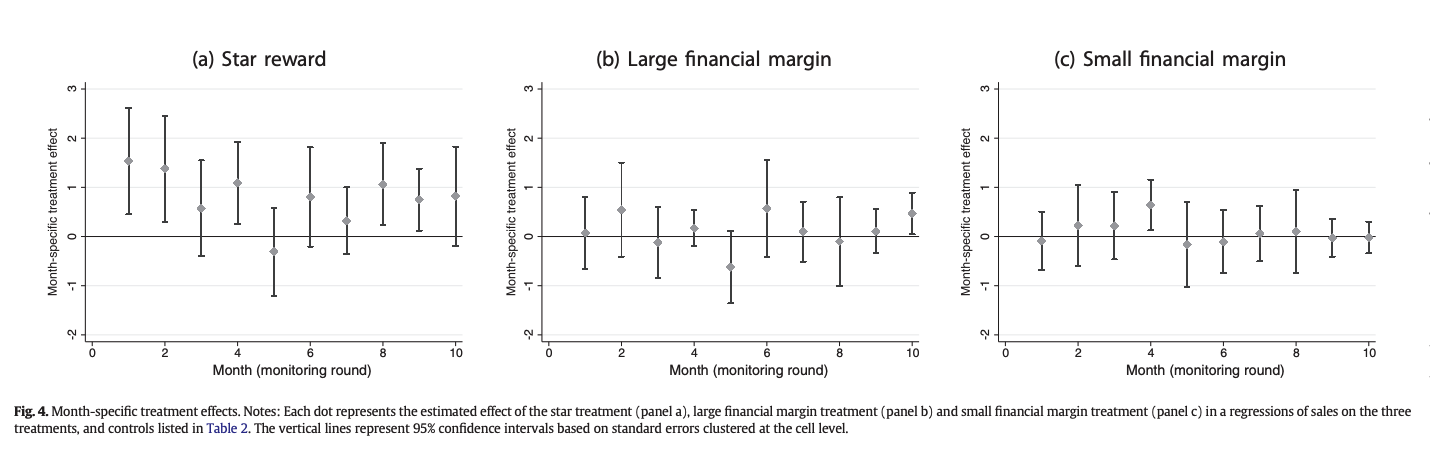
\includegraphics[width=\textwidth]{F4.png}
        \label{fig:my_label}
    \end{figure}
\end{frame}

\begin{frame}{Mechanisms: Increase in effort or demand?}
    \begin{figure}
        \centering
        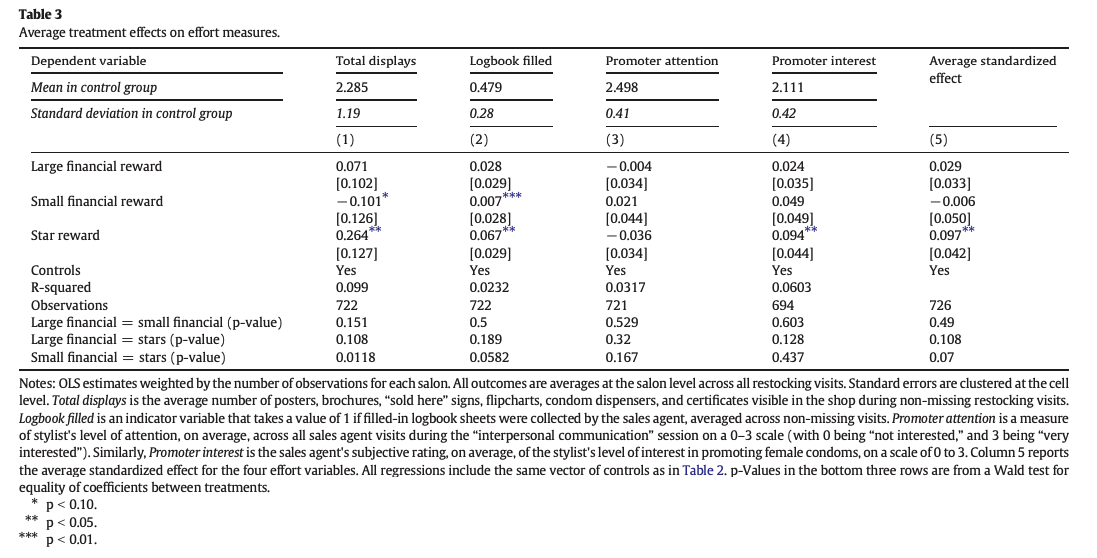
\includegraphics[width=\textwidth]{T3.png}
        \label{fig:my_label}
    \end{figure}
\end{frame}

\begin{frame}{Mechanisms: Increase in effort or demand?}
    \begin{figure}
        \centering
        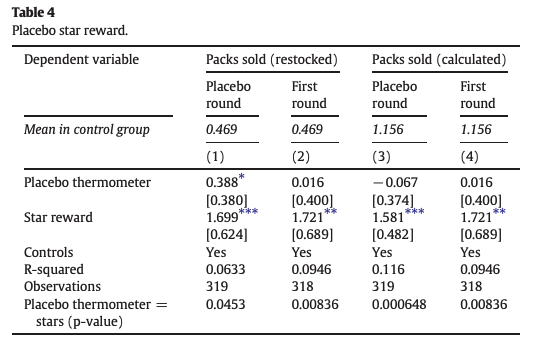
\includegraphics[width=\textwidth]{T4.png}
        \label{fig:my_label}
    \end{figure}
\end{frame}

\begin{frame}{Interaction between extrinsic and intristic motivation}
    \begin{figure}
        \centering
        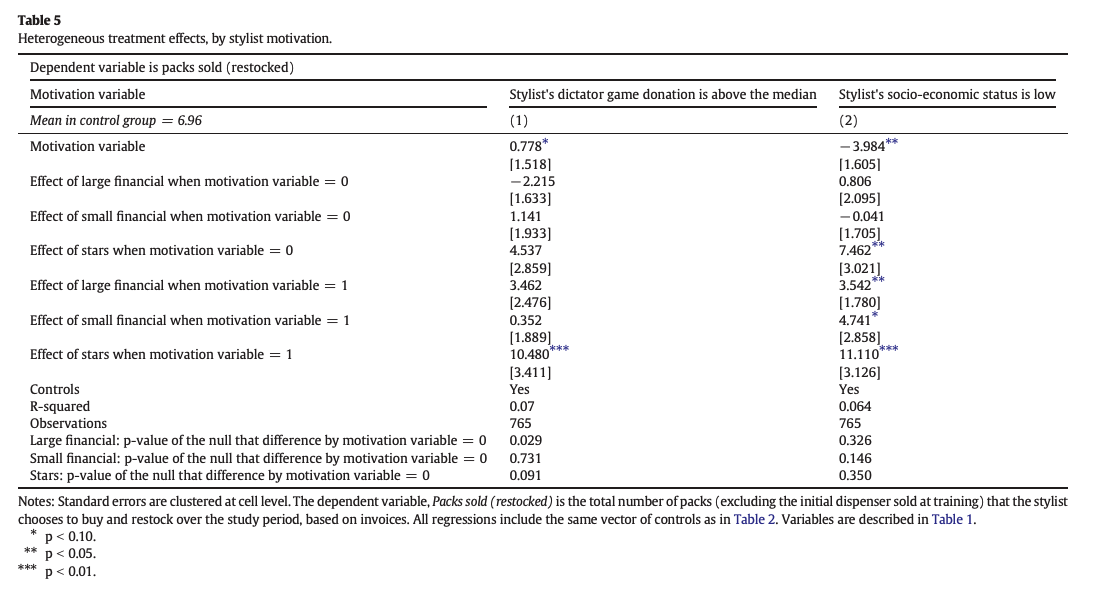
\includegraphics[width=\textwidth]{T5.png}
        \label{fig:my_label}
    \end{figure}
\end{frame}



\begin{frame}{Relative Value of Non-financial inventives}
    \begin{figure}
        \centering
        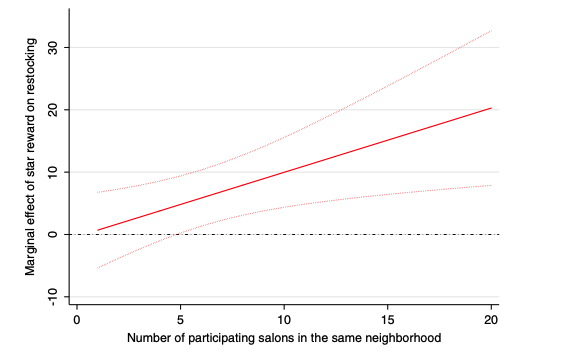
\includegraphics[width=\textwidth]{F5.png}
        \caption{Relative Value of Non-financial inventives}
        \label{fig:my_label}
    \end{figure}
\end{frame}

\begin{frame}{Discussion}
\begin{itemize}
    \item Very cool paper that takes a theoretical result/discussion where reality could be a little ambigious and tests it in the field.
    \item Question: What could be external validity of results? Could this result be peculiar to the sale of condoms? 
\end{itemize}

\end{frame}

\end{document}
